\section{Field-Programmable Gate Array (FPGA)} \label{sec:fpga}
%
%
As said in the Introduction, \acrshort{fpga} is a promising platform for the acceleration of \acrshort{cnn}s. According to \textcite{mittal_survey_2014}, \acrshort{fpga}s provide higher energy efficiency than both \acrshort{gpu}s and \acrshort{cpu} and a higher performance than \acrshort{cpu}s. Besides, \acrshort{fpga}s are very flexible hardware that can be tailored for each particular \acrshort{nn} \cite{vestias_fast_2019}. Furthermore, we can even expect that \acrshort{fpga}s will provide higher performance for performing \acrshort{cnn}s with respect to \acrshort{gpu} \cite{nurvitadhi_can_2017}.

According to \textcite{harris_digital_2015}, The definition of a \acrshort{fpga} is: \textquote{\textit{a \acrfull{fpga} is an array of reconfigurable gates}}. It is an integrated circuit that can implement combinatinal, sequential logic, and multilevel logic functions. An \acrshort{fpga} also integrates built-in multipliers, high-speed I/Os, data converters, large RAM arrays, and processors.

An illustration of a general \acrshort{fpga} layout can be found in Figure \ref{fig:fpga}. An \acrshort{fpga} is an array of configurable \acrfull{le}, also referred as \acrfull{clb}. Each \acrshort{le} can be configured to perform combinational or sequential logic and is connected to other \acrshort{le}s. The \acrshort{le}s array is connected to a set of \acrfull{ioe} to interface with the outside world.

A programmer can implement digital designs on the \acrshort{fpga} with a software programming tool, using either a \acrfull{hdl} or a schematic. An \acrshort{hdl} is a language to give the specifications of a digitial design. It allows a faster development cycle than schematic since we work at a higher level of abstraction. Moreover, the software is designed to optimize automatically the gates. The two leading \acrshort{hdl} are \textit{VHDL} and \textit{SystemVerilog}. They are build on the same principles and they mostly differ on the syntax.

%
The design flow of an \acrshort{fpga} can be described as follows: first the programmer creates the design by either a schematic or \acrshort{hdl}. Second, the design is synthesized, which means that the software determine how to configure the components of the \acrshort{fpga} in order to execute the specified function. Third, the software determines if the design is correct using a functional simulation. If it is correct, the software fits the element into the \acrshort{fpga} and does the \textbf{timing analysis}. This step simulates the real delay to check if the timing requirements are met. Finally, the design is programmed into the \acrshort{fpga} when the timing analysis simulation is correct.
%
\begin{figure}[H]
    \centering
    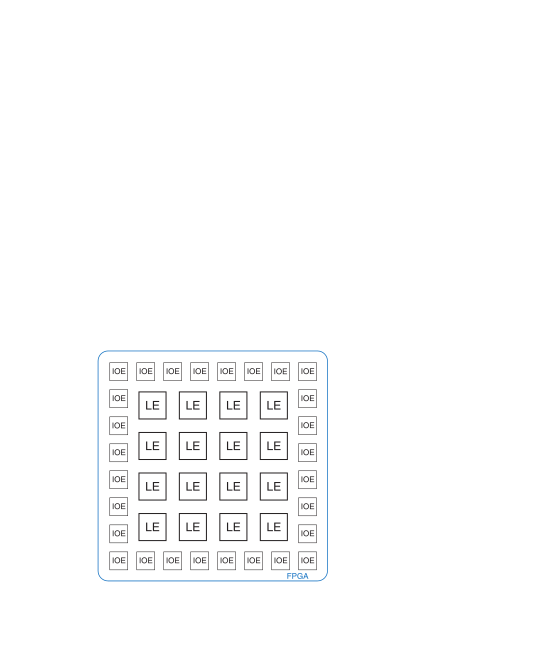
\includegraphics[width=0.5\textwidth]{fpga.pdf}
    \caption{General \acrshort{fpga} layout \cite{harris_digital_2015}}
    \label{fig:fpga}
\end{figure}
